\documentclass[11pt]{report}

\def\withcolors{1}
\def\withnotes{1}
\def\withindex{1}
\def\withbiblioconversion{1} % long names for the journals
%%%%%%%%%%%%%%%%%%%%%%%%%%%%%%%%%%%%%%%%%%%%%%%%%%%%%%%%%%%%%%%%%%%%%%%%%%%%%%%%%%%%
\usepackage[T1]{fontenc}
\usepackage[utf8]{inputenc}

%% Eye-candy
\usepackage{lmodern}
\usepackage{xspace}                                     % Smart spacing with \xspace
\usepackage[protrusion=true,expansion=true]{microtype}  % Improve font rendering

% Striking out text
\usepackage[normalem]{ulem}

%% Math
\usepackage{amsfonts,amsmath,amssymb, amsthm, mathtools}
\usepackage{thm-restate}
\usepackage{dsfont} % For the indicator symbol

% Algorithm environment
\usepackage{algorithmicx,algpseudocode,algorithm}

% Colors (with names)
\usepackage[usenames,dvipsnames,table]{xcolor}

% Quotes: \blockquote command
\usepackage{csquotes}

% Relative sizes for text
\usepackage{relsize}

% Bibliography
%\usepackage[numbers]{natbib}

% Required for the table of results
\usepackage{multirow}
\usepackage{chngpage} % allows for temporary adjustment of side margins

% For the commands such as \capitalisewords
\usepackage{mfirstuc}

% Graphics
\usepackage{tikz}
\usetikzlibrary{arrows}
\usetikzlibrary{calc,decorations.pathmorphing,patterns}

% For indexing
\ifnum\withindex=1
  \usepackage{makeidx}
  \usepackage{ifthen}
  \newcommand\indexed[2][]{\ifthenelse{\equal{#1}{}}{#2\index{#2}}{#2\index{#1}}}
  \makeindex %%%% Enable indexing
\fi
%%\usepackage{showidx} % To debug; does not play well with hyperref

% References and links
\usepackage[backref,colorlinks,citecolor=blue,bookmarks=true]{hyperref}
\usepackage{aliascnt}
\usepackage[numbered]{bookmark}

% Full pages
\usepackage{fullpage}

% Compressed lists
\usepackage[shortlabels]{enumitem}
  \setitemize{noitemsep,topsep=3pt,parsep=2pt,partopsep=2pt} % Uncomment for compact item lists
  \setenumerate{itemsep=1pt,topsep=2pt,parsep=2pt,partopsep=2pt}
  \setdescription{itemsep=1pt}
  
% Package for todo notes.
\ifnum\withnotes=1
  \usepackage[colorinlistoftodos,textsize=scriptsize]{todonotes}
\fi

% For testing and draft: to remove afterwards
\usepackage[english]{babel}
\usepackage{blindtext}

\makeatletter
\@ifundefined{theorem}{%
  % Theorems (each with its own style, all same counter). Cf. http://ftp.math.purdue.edu/mirrors/ctan.org/macros/latex/contrib/hyperref/doc/manual.pdf, p.17
  \theoremstyle{plain} %% Style
  	\newtheorem{theorem}{Theorem}[section]
  	\newaliascnt{coro}{theorem}
  	  \newtheorem{corollary}[coro]{Corollary}
  	\aliascntresetthe{coro}
  	\newaliascnt{lem}{theorem}
  		\newtheorem{lemma}[lem]{Lemma}
  	\aliascntresetthe{lem}
  	\newaliascnt{clm}{theorem}
  		\newtheorem{claim}[clm]{Claim}
	\aliascntresetthe{clm}
	\newaliascnt{fact}{theorem}
 	 	\newtheorem{fact}[theorem]{Fact}
	\aliascntresetthe{fact}
  	\newtheorem*{unnumberedfact}{Fact}
  \newaliascnt{prop}{theorem}
  		\newtheorem{proposition}[prop]{Proposition}
	\aliascntresetthe{prop}
	\newaliascnt{conj}{theorem}
  		\newtheorem{conjecture}[conj]{Conjecture}
	\aliascntresetthe{conj}
  \theoremstyle{remark} %% Style
  	\newtheorem{remark}[theorem]{Remark}
  	\newtheorem{question}[theorem]{Question}
  	\newtheorem*{notation}{Notation}
 	 \newtheorem{example}[theorem]{Example}
  \theoremstyle{definition} %% Style
  	\newaliascnt{defn}{theorem}
 		 \newtheorem{definition}[defn]{Definition}
 	 \aliascntresetthe{defn}
}{}
\makeatother
\providecommand*{\lemautorefname}{Lemma} % For \autoref{} to know the name of lemmas
\providecommand*{\clmautorefname}{Claim}
\providecommand*{\propautorefname}{Proposition}
\providecommand*{\coroautorefname}{Corollary}
\providecommand*{\defnautorefname}{Definition}
\newenvironment{proofof}[1]{\begin{proof}[Proof of {#1}]}{\end{proof}}

%% \email{} command
\providecommand{\email}[1]{\href{mailto:#1}{\nolinkurl{#1}\xspace}}

%% Remarks and notes
\ifnum\withcolors=1
  \newcommand{\new}[1]{{\color{red} {#1}}} % new
  \newcommand{\newer}[1]{{\color{blue} {#1}}} % even newer
  \newcommand{\newest}[1]{{\color{orange} {#1}}} % even even newer
  \newcommand{\newerest}[1]{{\color{blue!10!black!40!green} {#1}}} % you get the idea.
  \newcommand{\ccolor}[1]{{\color{RubineRed}#1}} % Clement
\else
  \newcommand{\new}[1]{{{#1}}}
  \newcommand{\newer}[1]{{{#1}}}
  \newcommand{\newest}[1]{{{#1}}}
  \newcommand{\newerest}[1]{{{#1}}}
  \newcommand{\ccolor}[1]{{#1}}
\fi

\ifnum\withnotes=1
  \newcommand{\cnote}[1]{\par\ccolor{\textbf{C: }\sf #1}} % Clement
  \newcommand{\todonote}[2][]{\todo[size=\scriptsize,color=red!40,#1]{#2}}  
	\newcommand{\questionnote}[2][]{\todo[size=\scriptsize,color=blue!30]{#2}}
	\newcommand{\todonotedone}[2][]{\todo[size=\scriptsize,color=green!40]{$\checkmark$ #2}}
	\newcommand{\todonoteinline}[2][]{\todo[inline,size=\scriptsize,color=orange!40,#1]{#2}}  
  \newcommand{\marginnote}[1]{\todo[color=white,linecolor=black]{{#1}}}
\else
  \newcommand{\cnote}[1]{{{#1}}}
  \newcommand{\todonote}[2][]{\ignore{#2}}
	\newcommand{\questionnote}[2][]{\ignore{#2}}
	\newcommand{\todonotedone}[2][]{\ignore{#2}}
	\newcommand{\todonoteinline}[2][]{\ignore{#2}}
  \newcommand{\marginnote}[1]{\ignore{#1}}
\fi
\newcommand{\ignore}[1]{\leavevmode\unskip} % eat unnecessary spaces before
\newcommand{\cmargin}[1]{\marginnote{\ccolor{#1}}} % Clement

% Shortcuts
\newcommand{\eps}{\ensuremath{\varepsilon}\xspace}
\newcommand{\Algo}{\ensuremath{\mathcal{A}}\xspace} % Algorithm A
\newcommand{\Tester}{\ensuremath{\mathcal{T}}\xspace} % Testing algorithm T
\newcommand{\Learner}{\ensuremath{\mathcal{L}}\xspace} % Learning algorithm L
\newcommand{\property}{\ensuremath{\mathcal{P}}\xspace} % Property P
\newcommand{\class}{\ensuremath{\mathcal{C}}\xspace} % Class C
\newcommand{\eqdef}{\stackrel{\rm def}{=}}
\newcommand{\eqlaw}{\stackrel{\mathcal{L}}{=}}
\newcommand{\accept}{\textsf{ACCEPT}\xspace}
\newcommand{\fail}{\textsf{FAIL}\xspace}
\newcommand{\reject}{\textsf{REJECT}\xspace}
\newcommand{\opt}{{\textsc{opt}}\xspace}
\newcommand{\half}{\frac{1}{2}}
\newcommand{\domain}{\ensuremath{\Omega}\xspace} % Domain of a distribution (default notation)
\newcommand{\distribs}[1]{\Delta\!\left(#1\right)} % Domain of a distribution (default notation)
\newcommand{\yes}{{\sf{}yes}\xspace}
\newcommand{\no}{{\sf{}no}\xspace}
\newcommand{\dyes}{{\cal Y}}
\newcommand{\dno}{{\cal N}}

% Complexity
\newcommand{\littleO}[1]{{o\mleft( #1 \mright)}}
\newcommand{\bigO}[1]{{O\mleft( #1 \mright)}}
\newcommand{\bigTheta}[1]{{\Theta\mleft( #1 \mright)}}
\newcommand{\bigOmega}[1]{{\Omega\mleft( #1 \mright)}}
\newcommand{\tildeO}[1]{\tilde{O}\mleft( #1 \mright)}
\newcommand{\tildeTheta}[1]{\operatorname{\tilde{\Theta}}\mleft( #1 \mright)}
\newcommand{\tildeOmega}[1]{\operatorname{\tilde{\Omega}}\mleft( #1 \mright)}
\providecommand{\poly}{\operatorname*{poly}}

% Influence
\newcommand{\totinf}[1][f]{{\mathbf{Inf}[#1]}}
\newcommand{\infl}[2][f]{{\mathbf{Inf}_{#1}(#2)}}
\newcommand{\infldeg}[3][f]{{\mathbf{Inf}_{#1}^{#2}(#3)}}

% Sets and indicators
\newcommand{\setOfSuchThat}[2]{ \left\{\; #1 \;\colon\; #2\; \right\} } 			% sets such as "{ elems | condition }"
\newcommand{\indicSet}[1]{\mathds{1}_{#1}}                                              % indicator function
\newcommand{\indic}[1]{\indicSet{\left\{#1\right\}}}                                             % indicator function
\newcommand{\disjunion}{\amalg}%\coprod, \dotcup...

% Distance
\newcommand{\dtv}{\operatorname{d_{\rm TV}}}
\newcommand{\totalvardist}[2]{{\dtv\!\left({#1, #2}\right)}}
\newcommand{\hellinger}[2]{{\operatorname{d_{\rm{}H}}\!\left({#1, #2}\right)}}
\newcommand{\kolmogorov}[2]{{\operatorname{d_{\rm{}K}}\!\left({#1, #2}\right)}}
\newcommand{\emd}[2]{{\operatorname{d_{\rm{}EMD}}\!\left({#1, #2}\right)}}
\newcommand{\dist}[2]{{\operatorname{dist}\!\left({#1, #2}\right)}}

% Restriction (functions, sequences, etc.)
\newcommand\restr[2]{{% we make the whole thing an ordinary symbol
  \left.\kern-\nulldelimiterspace % automatically resize the bar with \right
  #1 % the function
  \vphantom{\big|} % pretend it's a little taller at normal size
  \right|_{#2} % this is the delimiter
  }}

% Probability
\newcommand{\proba}{\Pr}
\newcommand{\probaOf}[1]{\proba\!\left[\, #1\, \right]}
\newcommand{\probaCond}[2]{\proba\!\left[\, #1 \;\middle\vert\; #2\, \right]}
\newcommand{\probaDistrOf}[2]{\proba_{#1}\left[\, #2\, \right]}

% Support of a distribution/function
\newcommand{\supp}[1]{\operatorname{supp}\!\left(#1\right)}

% Expectation & variance
\newcommand{\expect}[1]{\mathbb{E}\!\left[#1\right]}
\newcommand{\expectCond}[2]{\mathbb{E}\!\left[\, #1 \;\middle\vert\; #2\, \right]}
\newcommand{\shortexpect}{\mathbb{E}}
\newcommand{\var}{\operatorname{Var}}

% Distributions
\newcommand{\uniform}{\ensuremath{\mathcal{U}}}
\newcommand{\uniformOn}[1]{\ensuremath{\uniform\!\left( #1 \right) }}
\newcommand{\geom}[1]{\ensuremath{\operatorname{Geom}\!\left( #1 \right)}}
\newcommand{\bernoulli}[1]{\ensuremath{\operatorname{Bern}\!\left( #1 \right)}}
\newcommand{\bern}[2]{\ensuremath{\operatorname{Bern}^{#1}\!\left( #2 \right)}}
\newcommand{\binomial}[2]{\ensuremath{\operatorname{Bin}\!\left( #1, #2 \right)}}
\newcommand{\poisson}[1]{\ensuremath{\operatorname{Poisson}\!\left( #1 \right) }}
\newcommand{\gaussian}[2]{\ensuremath{ \mathcal{N}\!\left(#1,#2\right) }}
\newcommand{\gaussianpdf}[2]{\ensuremath{ g_{#1,#2}}}
\newcommand{\betadistr}[2]{\ensuremath{ \operatorname{Beta}\!\left( #1, #2 \right) }}

% Norms
\newcommand{\norm}[1]{\lVert#1{\rVert}}
\newcommand{\normone}[1]{{\norm{#1}}_1}
\newcommand{\normtwo}[1]{{\norm{#1}}_2}
\newcommand{\norminf}[1]{{\norm{#1}}_\infty}
\newcommand{\abs}[1]{\left\lvert #1 \right\rvert}
\newcommand{\dabs}[1]{\lvert #1 \rvert}
\newcommand{\dotprod}[2]{ \left\langle #1,\xspace #2 \right\rangle } 			% <a,b>
\newcommand{\ip}[2]{\dotprod{#1}{#2}} 			% shortcut

\newcommand{\vect}[1]{\mathbf{#1}} 			% shortcut

% Ceiling and floor
\newcommand{\clg}[1]{\left\lceil #1 \right\rceil}
\newcommand{\flr}[1]{\left\lfloor #1 \right\rfloor}

% Common sets
\newcommand{\R}{\ensuremath{\mathbb{R}}\xspace}
\newcommand{\C}{\ensuremath{\mathbb{C}}\xspace}
\newcommand{\Q}{\ensuremath{\mathbb{Q}}\xspace}
\newcommand{\Z}{\ensuremath{\mathbb{Z}}\xspace}
\newcommand{\N}{\ensuremath{\mathbb{N}}\xspace}
\newcommand{\cont}[1]{\ensuremath{\mathcal{C}^{#1}}}

% Oracles and variants
\newcommand{\ICOND}{{\sf INTCOND}\xspace}
\newcommand{\EVAL}{{\sf EVAL}\xspace}
\newcommand{\CDFEVAL}{{\sf CEVAL}\xspace}
\newcommand{\STAT}{{\sf STAT}\xspace}
\newcommand{\SAMP}{{\sf SAMP}\xspace}
\newcommand{\COND}{{\sf COND}\xspace}
\newcommand{\PCOND}{{\sf PAIRCOND}\xspace}
\newcommand{\ORACLE}{{\sf ORACLE}\xspace}

%% Terminology
\newcommand{\pdfsamp}{dual\xspace}
\newcommand{\cdfsamp}{cumulative dual\xspace}
\newcommand{\Pdfsamp}{\expandafter\capitalisewords\expandafter{\pdfsamp}}
\newcommand{\Cdfsamp}{\expandafter\capitalisewords\expandafter{\cdfsamp}}

% L_p norms
\newcommand{\lp}[1][1]{\ell_{#1}}

% Convolution
\DeclareMathOperator{\convolution}{\ast}

%% Terminology
\newcommand{\D}{\ensuremath{D}}
\newcommand{\distrD}{\ensuremath{\mathcal{D}}}
\newcommand{\birge}[2][\D]{\Phi_{#2}(#1)}
\newcommand{\iid}{i.i.d.\xspace}

% Sign
\DeclareMathOperator{\sign}{sgn}

%% Roman numerals
\makeatletter
\newcommand{\rom}[1]{\romannumeral #1}
\newcommand{\Rom}[1]{\expandafter\@slowromancap\romannumeral #1@}
\newcommand{\century}[2][th]{\Rom{#2}\textsuperscript{#1}}
\makeatother

% Hyperref and \autoref{} -- names
\renewcommand{\sectionautorefname}{Section} % To have "Section 5" instead of "section 5" with \autoref{}
\renewcommand{\chapterautorefname}{Chapter} % To have "Chapter 5" instead of "chapter 5" with \autoref{}
\renewcommand{\subsectionautorefname}{Section} % To have "Section 5" instead of "subsection 5" with \autoref{}
\renewcommand{\subsubsectionautorefname}{Section} % To have "Section 5" instead of "subsubsection 5" with \autoref{}
\def\algorithmautorefname{Algorithm}

\newcommand{\ket}[1]{|#1\rangle}
\newcommand{\bra}[1]{\langle #1|}
\def\twobytwomatrix[#1,#2,#3,#4]{
\begin{bmatrix}
	#1 & #2 \\
	#3 & #4
\end{bmatrix}
}

\def\dotproduct[#1,#2]{
\langle #1 | #2 \rangle
}
\newcommand{\transpose}[1]{{#1}^{\rm T}} 			% shortcut
\newcommand{\adjoint}[1]{{#1}^{\dagger}} 			% shortcut

%    Q-circuit version 2
%    Copyright (C) 2004  Steve Flammia & Bryan Eastin
%    Last modified on: 9/16/2011
%
%    This program is free software; you can redistribute it and/or modify
%    it under the terms of the GNU General Public License as published by
%    the Free Software Foundation; either version 2 of the License, or
%    (at your option) any later version.
%
%    This program is distributed in the hope that it will be useful,
%    but WITHOUT ANY WARRANTY; without even the implied warranty of
%    MERCHANTABILITY or FITNESS FOR A PARTICULAR PURPOSE.  See the
%    GNU General Public License for more details.
%
%    You should have received a copy of the GNU General Public License
%    along with this program; if not, write to the Free Software
%    Foundation, Inc., 59 Temple Place, Suite 330, Boston, MA  02111-1307  USA

% Thanks to the Xy-pic guys, Kristoffer H Rose, Ross Moore, and Daniel Müllner,
% for their help in making Qcircuit work with Xy-pic version 3.8.  
% Thanks also to Dave Clader, Andrew Childs, Rafael Possignolo, Tyson Williams,
% Sergio Boixo, Cris Moore, Jonas Anderson, and Stephan Mertens for helping us test 
% and/or develop the new version.

\usepackage{xy}
\xyoption{matrix}
\xyoption{frame}
\xyoption{arrow}
\xyoption{arc}

\usepackage{ifpdf}
\ifpdf
\else
\PackageWarningNoLine{Qcircuit}{Qcircuit is loading in Postscript mode.  The Xy-pic options ps and dvips will be loaded.  If you wish to use other Postscript drivers for Xy-pic, you must modify the code in Qcircuit.tex}
%    The following options load the drivers most commonly required to
%    get proper Postscript output from Xy-pic.  Should these fail to work,
%    try replacing the following two lines with some of the other options
%    given in the Xy-pic reference manual.
\xyoption{ps}
\xyoption{dvips}
\fi

% The following resets Xy-pic matrix alignment to the pre-3.8 default, as
% required by Qcircuit.
\entrymodifiers={!C\entrybox}

\newcommand{\braqc}[1]{{\left\langle{#1}\right\vert}}
\newcommand{\ketqc}[1]{{\left\vert{#1}\right\rangle}}
    % Defines Dirac notation. %7/5/07 added extra braces so that the commands will work in subscripts.
\newcommand{\qw}[1][-1]{\ar @{-} [0,#1]}
    % Defines a wire that connects horizontally.  By default it connects to the object on the left of the current object.
    % WARNING: Wire commands must appear after the gate in any given entry.
\newcommand{\qwx}[1][-1]{\ar @{-} [#1,0]}
    % Defines a wire that connects vertically.  By default it connects to the object above the current object.
    % WARNING: Wire commands must appear after the gate in any given entry.
\newcommand{\cw}[1][-1]{\ar @{=} [0,#1]}
    % Defines a classical wire that connects horizontally.  By default it connects to the object on the left of the current object.
    % WARNING: Wire commands must appear after the gate in any given entry.
\newcommand{\cwx}[1][-1]{\ar @{=} [#1,0]}
    % Defines a classical wire that connects vertically.  By default it connects to the object above the current object.
    % WARNING: Wire commands must appear after the gate in any given entry.
\newcommand{\gate}[1]{*+<.6em>{#1} \POS ="i","i"+UR;"i"+UL **\dir{-};"i"+DL **\dir{-};"i"+DR **\dir{-};"i"+UR **\dir{-},"i" \qw}
    % Boxes the argument, making a gate.
\newcommand{\meter}{*=<1.8em,1.4em>{\xy ="j","j"-<.778em,.322em>;{"j"+<.778em,-.322em> \ellipse ur,_{}},"j"-<0em,.4em>;p+<.5em,.9em> **\dir{-},"j"+<2.2em,2.2em>*{},"j"-<2.2em,2.2em>*{} \endxy} \POS ="i","i"+UR;"i"+UL **\dir{-};"i"+DL **\dir{-};"i"+DR **\dir{-};"i"+UR **\dir{-},"i" \qw}
    % Inserts a measurement meter.
    % In case you're wondering, the constants .778em and .322em specify
    % one quarter of a circle with radius 1.1em.
    % The points added at + and - <2.2em,2.2em> are there to strech the
    % canvas, ensuring that the size is unaffected by erratic spacing issues
    % with the arc.
\newcommand{\measure}[1]{*+[F-:<.9em>]{#1} \qw}
    % Inserts a measurement bubble with user defined text.
\newcommand{\measuretab}[1]{*{\xy*+<.6em>{#1}="e";"e"+UL;"e"+UR **\dir{-};"e"+DR **\dir{-};"e"+DL **\dir{-};"e"+LC-<.5em,0em> **\dir{-};"e"+UL **\dir{-} \endxy} \qw}
    % Inserts a measurement tab with user defined text.
\newcommand{\measureD}[1]{*{\xy*+=<0em,.1em>{#1}="e";"e"+UR+<0em,.25em>;"e"+UL+<-.5em,.25em> **\dir{-};"e"+DL+<-.5em,-.25em> **\dir{-};"e"+DR+<0em,-.25em> **\dir{-};{"e"+UR+<0em,.25em>\ellipse^{}};"e"+C:,+(0,1)*{} \endxy} \qw}
    % Inserts a D-shaped measurement gate with user defined text.
\newcommand{\multimeasure}[2]{*+<1em,.9em>{\hphantom{#2}} \qw \POS[0,0].[#1,0];p !C *{#2},p \drop\frm<.9em>{-}}
    % Draws a multiple qubit measurement bubble starting at the current position and spanning #1 additional gates below.
    % #2 gives the label for the gate.
    % You must use an argument of the same width as #2 in \ghost for the wires to connect properly on the lower lines.
\newcommand{\multimeasureD}[2]{*+<1em,.9em>{\hphantom{#2}} \POS [0,0]="i",[0,0].[#1,0]="e",!C *{#2},"e"+UR-<.8em,0em>;"e"+UL **\dir{-};"e"+DL **\dir{-};"e"+DR+<-.8em,0em> **\dir{-};{"e"+DR+<0em,.8em>\ellipse^{}};"e"+UR+<0em,-.8em> **\dir{-};{"e"+UR-<.8em,0em>\ellipse^{}},"i" \qw}
    % Draws a multiple qubit D-shaped measurement gate starting at the current position and spanning #1 additional gates below.
    % #2 gives the label for the gate.
    % You must use an argument of the same width as #2 in \ghost for the wires to connect properly on the lower lines.
\newcommand{\control}{*!<0em,.025em>-=-<.2em>{\bullet}}
    % Inserts an unconnected control.
\newcommand{\controlo}{*+<.01em>{\xy -<.095em>*\xycircle<.19em>{} \endxy}}
    % Inserts a unconnected control-on-0.
\newcommand{\ctrl}[1]{\control \qwx[#1] \qw}
    % Inserts a control and connects it to the object #1 wires below.
\newcommand{\ctrlo}[1]{\controlo \qwx[#1] \qw}
    % Inserts a control-on-0 and connects it to the object #1 wires below.
\newcommand{\targ}{*+<.02em,.02em>{\xy ="i","i"-<.39em,0em>;"i"+<.39em,0em> **\dir{-}, "i"-<0em,.39em>;"i"+<0em,.39em> **\dir{-},"i"*\xycircle<.4em>{} \endxy} \qw}
    % Inserts a CNOT target.
\newcommand{\qswap}{*=<0em>{\times} \qw}
    % Inserts half a swap gate.
    % Must be connected to the other swap with \qwx.
\newcommand{\multigate}[2]{*+<1em,.9em>{\hphantom{#2}} \POS [0,0]="i",[0,0].[#1,0]="e",!C *{#2},"e"+UR;"e"+UL **\dir{-};"e"+DL **\dir{-};"e"+DR **\dir{-};"e"+UR **\dir{-},"i" \qw}
    % Draws a multiple qubit gate starting at the current position and spanning #1 additional gates below.
    % #2 gives the label for the gate.
    % You must use an argument of the same width as #2 in \ghost for the wires to connect properly on the lower lines.
\newcommand{\ghost}[1]{*+<1em,.9em>{\hphantom{#1}} \qw}
    % Leaves space for \multigate on wires other than the one on which \multigate appears.  Without this command wires will cross your gate.
    % #1 should match the second argument in the corresponding \multigate.
\newcommand{\push}[1]{*{#1}}
    % Inserts #1, overriding the default that causes entries to have zero size.  This command takes the place of a gate.
    % Like a gate, it must precede any wire commands.
    % \push is useful for forcing columns apart.
    % NOTE: It might be useful to know that a gate is about 1.3 times the height of its contents.  I.e. \gate{M} is 1.3em tall.
    % WARNING: \push must appear before any wire commands and may not appear in an entry with a gate or label.
\newcommand{\gategroup}[6]{\POS"#1,#2"."#3,#2"."#1,#4"."#3,#4"!C*+<#5>\frm{#6}}
    % Constructs a box or bracket enclosing the square block spanning rows #1-#3 and columns=#2-#4.
    % The block is given a margin #5/2, so #5 should be a valid length.
    % #6 can take the following arguments -- or . or _\} or ^\} or \{ or \} or _) or ^) or ( or ) where the first two options yield dashed and
    % dotted boxes respectively, and the last eight options yield bottom, top, left, and right braces of the curly or normal variety.  See the Xy-pic reference manual for more options.
    % \gategroup can appear at the end of any gate entry, but it's good form to pick either the last entry or one of the corner gates.
    % BUG: \gategroup uses the four corner gates to determine the size of the bounding box.  Other gates may stick out of that box.  See \prop.

\newcommand{\rstick}[1]{*!L!<-.5em,0em>=<0em>{#1}}
    % Centers the left side of #1 in the cell.  Intended for lining up wire labels.  Note that non-gates have default size zero.
\newcommand{\lstick}[1]{*!R!<.5em,0em>=<0em>{#1}}
    % Centers the right side of #1 in the cell.  Intended for lining up wire labels.  Note that non-gates have default size zero.
\newcommand{\ustick}[1]{*!D!<0em,-.5em>=<0em>{#1}}
    % Centers the bottom of #1 in the cell.  Intended for lining up wire labels.  Note that non-gates have default size zero.
\newcommand{\dstick}[1]{*!U!<0em,.5em>=<0em>{#1}}
    % Centers the top of #1 in the cell.  Intended for lining up wire labels.  Note that non-gates have default size zero.
\newcommand{\Qcircuit}{\xymatrix @*=<0em>}
    % Defines \Qcircuit as an \xymatrix with entries of default size 0em.
\newcommand{\link}[2]{\ar @{-} [#1,#2]}
    % Draws a wire or connecting line to the element #1 rows down and #2 columns forward.
\newcommand{\pureghost}[1]{*+<1em,.9em>{\hphantom{#1}}}
    % Same as \ghost except it omits the wire leading to the left. 
 % To draw quantum circuits in LaTeX

\newcommand{\complex}{\textsf{com}\xspace}
\newcommand{\integ}{\textsf{int}\xspace}
\newcommand{\float}{\textsf{float}\xspace}
\newcommand{\mat}{\textsf{mat}\xspace}

\newcommand{\QL}{\textsf{QLang}\xspace}
\title{\QL: Qubit Language\\ \Large(Final Report)}
\author{
  Christopher Campbell
  \and Cl\'ement Canonne
  \and Sankalpa Khadka
  \and Winnie Narang
  \and Jonathan Wong
}

\begin{document}

\maketitle
\tableofcontents

\ifnum\withnotes=1
  \listoftodos
\fi

\chapter{An Introduction to the Language}
  The \QL language is a scientific tool that enables easy and simple simulation of quantum computing on classical computers. 
Featuring a clear and intuitive syntax, \QL makes it possible to take any quantum algorithm and implement it seamlessly, while 
conserving both the overall structure and syntactical features of the original pseudocode. The \QL code is then compiled to 
C++, allowing for an eventual high-performance execution -- a process made simple and transparent to the user, who can focus on
the algorithmic aspects of the quantum simulation.
\section{Background: Quantum Computing}

In classical computing, data are stored in the form of binary digits or bits. A \emph{bit} is the basic unit of information stored and manipulated in a computer, which in one of two possible distinct states (for instance: two distinct voltages, on and off state of electric switch, two directions of magnetization, etc.). 
The two possible values/states of a system are represented as binary digits, $0$ and $1$. In a quantum computer, however, data are stored in the form of \emph{qubits}, or quantum bits. A quantum system of $n$ qubits is a Hilbert space of dimension $2^n$; fixing any orthonormal basis, any \emph{quantum state} can thus be uniquely written as a linear combination of $2^n$ orthogonal vectors $\{\ket{i}\}_i$ where $i$ is an $n$-bit binary number.

\begin{example}A $3$ qubit system has a canonical basis of 8 orthonormal states denoted 
$\ket{000}$, $\ket{001}$, $\ket{010}$, $\ket{011}$, $\ket{100}$, $\ket{101}$, $\ket{110}$, $\ket{111}$.
\end{example}
To put it briefly, while a classical bit has only two states (either $0$ or $1$), a qubit can have  states $\ket{0}$ and $\ket{1}$, or any linear combination of states also known as a \emph{superposition}: %. Hence, a qubit can have an infinitely many states,
\[
	\ket{\phi}=\alpha\ket{0}+\beta\ket{1}
\]
where $\alpha,\beta\in\C$ are any complex numbers such that $\abs{\alpha}^2+\abs{\beta}^2=1$.\medskip

Similarly, one may recall that logical operations, also known as \emph{logical gates}, are the basis of computation in classical computers. Computers are built with circuit that is made up of logical gates. The examples of logical gates are \textsf{AND}, \textsf{OR}, \textsf{NOT}, \textsf{NOR}, \textsf{XOR}, etc. The analogue for quantum computers, \emph{quantum gates}, are operations which are a \emph{unitary transformation} on qubits. The quantum gates are represented by matrices, and a gate acts on $n$ qubits is represented by $2^n \times 2^n$ unitary matrix\footnote{That is, a matrix $U\in\C^{2^n\times 2^n}$ such that $\adjoint{U}U=I_{2^n}$, where $\adjoint{\cdot}$ denotes the Hermitian conjugate.}. Analogous to the classical computer which is built from an electrical circuit containing wires and logic gates, quantum computers are built from  quantum circuits containing ``wires'' and quantum gates to carry out the computation.\medskip

\noindent More on this, as well as the definition of the usual quantum gates, can be found in \autoref{app:quantum:more}.

\subsection {Dirac notation for quantum computation}
In quantum computing, \emph{Dirac notation} is generally used to represent qubits. This notation provides concise and intuitive representation of complex matrix operations.

More precisely, a column vector $\left[ \begin {array} {c} c_1\\ c_2\\ \vdots\\ c_n \end{array} \right]$ is represented as $\ket{\psi}$, also read as ``ket psi''.  In particular, the computational basis states, also know as \emph{pure states} are represented as $\ket{i}$  where  $i$ is a $n$-bit binary number. For example,
\[
\ket{000}=\begin{bmatrix} 1\\ 0\\ 0\\ 0\\ 0\\ 0\\ 0\\ 0 \end{bmatrix},
\ket{001}=\begin{bmatrix} 0\\ 1\\ 0\\ 0\\ 0\\ 0\\ 0\\ 0 \end{bmatrix},
\ket{010}=\begin{bmatrix} 0\\ 0\\ 1\\ 0\\ 0\\ 0\\ 0\\ 0 \end{bmatrix},
\dots,
\ket{101}=\begin{bmatrix} 0\\ 0\\ 0\\ 0\\ 0\\ 1\\ 0\\ 0 \end{bmatrix},
\ket{110}=\begin{bmatrix} 0\\ 0\\ 0\\ 0\\ 0\\ 0\\ 1\\ 0 \end{bmatrix},
\ket{111}=\begin{bmatrix} 0\\ 0\\ 0\\ 0\\ 0\\ 0\\ 0\\ 1 \end{bmatrix}
\]
Similarly, the row vector $\begin{bmatrix} c^\ast_1 & c^\ast_2  & \dots & c^\ast_n & \end{bmatrix}$, which is also complex conjugate transpose of $\ket{\psi}$, is represented as $\bra{\psi}$, also read as ``bra psi''.\medskip

The inner product of vectors $\ket{\varphi}$ and $\ket{\psi}$ is written $\dotprod{ \varphi }{ \psi }$.
The tensor product of vectors $\ket{\varphi}$ and $\ket{\psi}$ is written $\ket{\varphi} \otimes \ket{\psi}$  and more commonly $\ket{\varphi}\ket{\psi}$.
We list below a few other mathematical notions that are relevant in quantum computing:

\begin{itemize}[-]
\item $z^\ast$ (complex conjugate of elements)\\  if $z=a+ib$, then $z^\ast = a - ib$.
\item $A^\ast$ (complex conjugate of matrices)\\ if $A = \twobytwomatrix[1,6i,3i,2+4i]$ then $A^\ast = \twobytwomatrix[1,-6i,-3i,2-4i]$.
%%%%%%%%%%%%%%%%%%%%%% Transpose of A
\item $\transpose{A}$  (transpose of matrix $A$)\\ if $A = \twobytwomatrix[1,6i,3i,2+4i]$ then $\transpose{A} = \twobytwomatrix[1,3i,6i,2+4i]$.
%%%%%%%%%%%%%%%%%%%%%% Adjoint of A
\item $\adjoint{A}$  (Hermitian conjugate (adjoint) of matrix $A$)\\
Defined as $\adjoint{A} = \left(\transpose{A}\right)^\ast$; if $A = \twobytwomatrix[1,6i,3i,2+4i]$ then $A^{\dag} = \twobytwomatrix[1,-3i,-6i,2-4i]$
%%%%%%%%%%%%%%%%%%%%%% Norm
\item $\norm{\ket{\psi}}$ ($\lp[2]$ norm of vector $\ket{\psi}$)\\
$\norm{\ket{\psi}} = \sqrt{\dotproduct[{\psi}, {\psi}]}$. 
 (This is often used to normalize $\ket{\psi}$ into a unit vector $\frac{\ket{\psi}}{\norm{\ket{\psi}}}$.)
%%%%%%%%%%%%%%%%%%%%%% Other

\item $\bra{\varphi}A\ket{\psi}$ (inner product of $\ket{\varphi}$ and $A\ket{\psi}$). \\
Equivalently\footnote{Recall that we work in a complex Hilbert space: the inner product is a sesquilinear form.}, inner product of $A^{\dag}\ket{\varphi}$ and $\ket{\psi}$

\end{itemize}

\subsection{Quantum Algorithms}
A quantum algorithm is an algorithm that, in addition to operations on bits, can apply quantum gates to qubits and measure the outcome, in order to perform a computation or solve a search problem. Inherently, the outcome of such algorithms will be probabilistic: for instance, a quantum algorithm is said to \emph{compute a function $f$ on input $x$} if, for all $x$, the value $f(x)$ it outputs is correct with high probability.
  The representation of a quantum computation process requires an input register, output register and unitary transformation that takes a computational basis states into linear combination of computational basis states. If $x$ represents an $n$ qubit input register and $y$ represents an $m$ qubit output register, then the effect of a unitary transformation $U_f$ on the computational basis $\ket{x}_n\ket{y}_m$ is represented as follows:
	\begin{equation}
	U_f(\ket{x}_n\ket{y}_m)=\ket{x}_n\ket{y\oplus f(x)}_m,
	\end{equation}
	where $f$ is a function that takes an $n$ qubit input register and returns an $m$ qubit output and $\oplus$ represents mod-$2$ bitwise addition.


\section{Related Work}

\todo{Fill the related work here. Other languages, etc.}
\section{Goal and objectives}

\QL has been designed with a handful of key characteristics in mind:
\begin{description}
  \item[Intuitive.] Any student or researcher familiar with quantum computing should be able to transpose and implement their algorithms easily and quickly, without wasting time struggling to udnerstand idiosyncrasies of the language. 
  \item[Specific.] The language has one purpose -- implementing quantum algorithms. Anything that is not related to nor useful for this purpose should not be -- and is not -- part of \QL (e.g., the language does not support strings).
  \item[Simple.] Matrices, vector operations are pervasive in quantum computing -- thus, they must be easy to use and understand. All predefined structures and functions are straightforward to use, and have no puzzling nor counter-intuitive behavior.
\end{description}
In a nutshell, \QL is simple, includes everything it should -- and nothing it should not.

\chapter{\QL in practice: a Tutorial}
  \section{Basics and syntax}

A \QL file (extension \texttt{.ql} by convention) comprises several functions, each of them having its own variables. Once compiled, a program will start by calling the \textsf{compute()} function that must appear in the \texttt{.ql} file, and whose prototype is as follows:
\begin{lstlisting}
def compute(int a): int trial {
  # do some stuff, call some other functions
}
\end{lstlisting}
In particular, the main entry point \textsf{compute()} receives an integer argument, \textsf{a}, and returns an integer value, \textsf{type}.
Note also that \QL is case-sensitive: \textsf{compute} and \textsf{Compute} would be two different functions (however, indentation is completely unrestricted).

As hinted above, comments in the language are single-line, and start with a \#: everything following this symbol, until the next line return, will be ignored by the compiler. Furthermore, a function is defined (and declared -- there is no forward declaration) by the keyword \textsf{def} followed by the details of the function:
\begin{lstlisting}
def function_name(type1 param1, type2 param2, ..., typek paramk): type returnvar {
  # variable declarations
  # body of the function
}
\end{lstlisting}
The valid types  in \QL for parameters, return variables and variables are \texttt{int}, \texttt{float}, \texttt{comp}, \texttt{mat}: respectively integers, real numbers, complex numbers and matrices (the latter including, as we shall see, qubits). In the above, the return variable \textsf{returnvar} is available in the body of the function, and its value will be returned at the end of the function call. All other local variables must be declared, one by line, at the beginning of the function body: in particular, it is not possible to mix variable declaration and assignment:
\begin{lstlisting}
def foo( mat bar ): mat blah {
  int bleh;                       # OK
  int bluh = 0;                   # Not OK: parsing error
  comp blih, bloh;                # Not OK: one variable at a time
  bleh = 5;                       # OK
  bleh = bleh+1                   # Not OK: missing semicolon
  bleh = bleh * 4 +
         2^bleh;                  # OK: statements can span several lines
  bleh = bleh-1; bleh = 2*bleh;   # OK: several statements per line
  blah = bleh * bar;              # OK: blah is the returned variable
}
\end{lstlisting}
As examplified above, each statement (declaration, assignment, operation) can span any number of lines, and end with a semicolon.

\paragraph{Qubits, matrices and vectors.} Before turning to the flow control structures, recall that \QL is designed specifically for the sake of implementing quantum algorithms; as such, it supports the usual quantum notations for bra and kets (although it stores and recognize then as of type \textsf{mat}):
\begin{lstlisting}
  mat idt;
  mat vct;
  mat qub;
  qub = |11>;            # this is a bra
  qub = <01|;            # this is a ket
  idt = [(1,0)(0,1)];    # this is a matrix
  vct = [(1,2,C(3.2 + 1.I))];   # this is a vector (with complex entries)
  vct = qub;             # this is OK
\end{lstlisting}
In the above, the 3 variables have the same type -- the difference is only syntatical, in order to provide the user with an intuitive way to program the quantum operations.


\section{Control structures, built-in functions and conversions}
Now that the basic syntax of the language has been described, it is time to have a look at the fundamental blocks of any algorithm: the control structures, such as loops and conditional statements. 

\paragraph{Loops.} \QL supports two sorts of loop, the \textsf{for} and \textsf{while} statements. While their bahavior is illustrated below, it is important to remember two features of the \textsf{for} loop: namely, that \textsf{(a)} the loop index must be a variable declared beforehand; and \textsf{(b)} that the (optional) keyword \textsf{by} allows to set the increment size by any integer, even negative.

\begin{lstlisting}
 int i; # Will be used as 'for' loop index
 int a;

 for( i from 0 to 2 by 1 ) # OK
   a=a+5;

 for( i from 2 to 0 by -1 ) # OK
 {
     a=a*10;
     continue; # going to next iteration: the next instruction will never be executed.
     print(a);
 }
 
 for( i from 1 to 10 ) # OK: missing "by 1" is implicit
 {
     a=a-3;
     break; # For the sake of the example: leaves the loop.
 }
 
 while( a leq 10 ) # OK
 a=a+1;
 
 while( a neq 0 )  # OK
 {
     a = (a+1) % 42;
     continue;
     print(0); # never reached
 }
\end{lstlisting}
As shown above, braces are optional when the body of the loop comprises only one line.

\paragraph{Conditional constructs.} As in many languages, \QL supports a C-like \textsf{if}\dots\textsf{else} construct:
\begin{lstlisting}
       if( predicate )
       {
          # Do something
       }
       else
       {
          # Do something else
       }
\end{lstlisting}
The predicate can be any expression evaluating to an integer: if non-zero, the \textsf{if} statement is entered; otherwise, the (optional) \textsf{else} statement is entered, if it exists. Note that \QL does not provide a builtin construct \textsf{elseif}, but instead relies on a nested combination of \textsf{if} and \textsf{else}:
\begin{lstlisting}
 if(z eq 5) a = 0;
       
 a = a - 2;
 if( z leq 5 )
 {
    a = 0;
 }
 else
 {
    a = 10;
    b = 24;
 }
       
 if( a gt 100 )
 {
    print(b); # a > 100
 }
 else if( a eq 10 )
 {
    print(a);
 }
\end{lstlisting}

\paragraph{Builtin functions and operators.} As shown in the previous two examples, \QL provides builtin constructs to perform basic or fundamental tasks:
\begin{description}
  \item[\rm\em Comparison operators:] \textsf{gt}, \textsf{lt}, \textsf{geq}, \textsf{leq}, \textsf{eq}, \textsf{neq} take two operands $a$, $b$, and return 0 (resp. 1) if respectively $a > b$, $a < b$, $a \geq b$, $a \leq b$, $a \leq b$ and $a = b$ and $a \neq b$;
  \item[\rm\em Builtin functions:] these are convenient functions such as \textsf{print}, \textsf{printq} (for qubit syntax), or mathematical ones applying to matrices such as \textsf{norm}, \textsf{adj}, to complex values ($\textsf{sin}$, $\textsf{im}$, \dots) or to $0/1$ integers (``Booleans'') such as \textsf{and}, \textsf{xor}.
  \item[\rm\em Operators:] the language supports the usual unary (negation $-$, logical negation $\textsf{not}$), binary (addition $+$, substraction $-$, exponentiation $\hat{}$ \dots) operators, as well as some more specific ones (tensor product $@$).
%  \item[\rm\em Constants:] \todonote{fill in}
\end{description}
The complete list of these functions, operators and builtin constants can be found in \autoref{sec:reference}.

\paragraph{Implicit conversions.} 
Implicit conversions for some operators such as \textsf{eq} is possible, according to the following rule: \texttt{int}$\leadsto$\texttt{float}$\leadsto$\texttt{comp}$\leadsto$\texttt{mat}. However, the language is otherwise strongly typed: it is not possible to assign a complex number to a variable of type $\texttt{mat}$, for instance.

\todo{Do we support recursive functions?}

\section{Diving in: Deutsch--Jozsa Algorithm}

To illustrate and describe the process of writing in \QL, this section will walk the reader through the implementation of one of the most emblematic quantum examples, namely \emph{Deutsch-Jozsa Algorithm}. The goal of this algorithm is to answer the following question: given query access to an unknown fucntion $f\colon\{0,1\}^n \to \{0,1\}$, promised to be either constant or balanced\footnote{$f$ is said to be balanced if $f(x)=0$ for exactly half of the inputs $x\in\{0,1\}^n$; or, equivalently, if $\shortexpect_{x}[f(x)] = \frac{1}{2}$.}, which of the two holds?  Classically, it is easy to see that this requires (in the worst case) querying just over half the solution space, that is $2^{n-1} + 1$ queries.  Quantumly, the Deutsch-Jozsa algorithm enables us to answer this question with just \emph{one} query!\medskip

\noindent The circuit performing the algorithm is given below:
\begin{align*}
 \Qcircuit @C=1em @R=.7em {
  \lstick{\ket{0}} & /^n \qw & \gate{H^{\otimes n}} & \multigate{1}{U_f} & \gate{H^{\otimes n}}	& \meter & \cw \\
  \lstick{\ket{1}} & \qw     & \gate{H}             & \ghost{U_f}        & \qw
 }
\end{align*}

To implement it in \QL, we first have to implement the $n$-fold Hadamard gate $H^{\otimes n}$; recalling that the Hadamard gate $H$ is a built-in operator of the language, this can be done as follows:\todonote{Check the QL code for Deutsch-Jozsa -- there were typos and mistakes in the .ql file.}
\begin{lstlisting}
  def hadamard(int n): mat gate{
        #returns Hadamard gate of 2^n dimensions
        gate = H; 
        for(i from 1 to n by 1){
                gate = gate @ H;                 
        }       
}
\end{lstlisting}
Now, to implement the measurement gate (or, more precisely, to return the measurement matrix), we write the following code that takes a ket $\ket{x}$ and returns the matrix $\ket{x}\bra{x}$:
\begin{lstlisting}
def measure(qubk top): mat result{
        # returns the measurement matrix  
        mat adjoint = Adj(top);
        result = top * adjoint;
}
\end{lstlisting}
(Note that $\ket{x}\bra{x}$ was written as $\ket{x}\operatorname{adjoint}(\ket{x})$, which is performed above using the transparent conversion between vectors and matrices provided by the language.)\medskip

Once all the ``building blocks'' (gates) of the algorithm have been implemented, we can write down the algorithm \emph{as it appears from the circuit above}: the function takes as argument a qubit \textsf{top} (in the diagram, $\ket{0}$), the parameter size $n$, as well as the unitary matrix implementing the quantum  gate $U_f$ (the access to the unknown function $f$), and returnings either 0 or 1, dependeing one wether the function is constant or balanced.
\begin{lstlisting}
def deutsch(int n, qubk top, mat U): int outcomeZero{       
        qubk bottom;  # originally, the |1> qubit    
        mat input; # input will be the tensor product of top and bottom register  
        mat had;   # n-fold Hadamard gate  
        mat meas;

        bottom = |1>;
        input = top @ bottom;
        had = hadamard(n);
        input = had * input;
        
        input = U*input;
        input = (H @ I)*input;
        
        meas = measure (top);        
        input = ((meas@I)*input;
        
        input = norm(input);
        
        if (eq(input,0)){
                outcomeZero = 0;
        }
        else{
                outcomeZero = 1;
        }
}
\end{lstlisting}

Finally, we can call (and test) our algorithm by defining two unitary transformations (here $U_b$ and $U_c$) and testing our function on them -- and print the output. This is done by writing the entry point function, \textsf{compute}:
\begin{lstlisting}
def compute (): int outcome{
        qubk top;
        mat Ub;
        mat Uc;
        int n;
        
        n = 1;
        top = |0>;
        Ub = [(1,0,0,0)(0,1,0,0)(0,0,0,1)(0,0,1,0)];
        Uc = [(1,0,0,0)(0,1,0,0)(0,0,1,0)(0,0,0,1)]; # identity

        outcome = deutsch (2,top, Ub);
        print(outcome);
        outcome = deutsch (2,top, Uc);
        print(outcome);
}
\end{lstlisting}


\todo[inline]{Other algorithms?}

\chapter{Reference Manual}\label{sec:reference}
  
\section{Lexical conventions}
There are five kinds of tokens: identifiers, keywords, constants, expression operators, and other separators. There are six kinds of tokens: identifiers, keywords, constants, strings, expression operators, and other separators. If the input stream has been parsed into tokens up to a given character, the next token is taken to include the longest string of characters which could possibly constitute a token.\cmargin{Rephrase: that's plagiarism}

\section{Character set}
\QL supports a subset of ASCII; that is, allowed characters are
\fbox{\texttt{a-zA-Z0-9\#,.-\_;:()[]\{\}<>=+/|*@}}, as well as tabulations \texttt{\textbackslash{}t}, spaces, and line returns \texttt{\textbackslash{}n} and {\textbackslash{}r}.
\section{Comments}
Comments start with a \# sign, which then extends until the next carriage return. Multiline comments are not supported.

\section{Identifier (names)}
An identifier is an arbitrarily long sequence of alphabetic and numeric characters, where \texttt{\_} is included as ``alphabetic''. It must start with a lowercase or uppercase letter, i.e. one of $\texttt{a-zA-Z}$.

\noindent The language is case-sensitive: \texttt{hullabaloo} and \texttt{hullABaLoo} are considered as different.

An operation, or language elementary unit, starts from the end of the previous one, and ends whenever a semicolon (that is not part of a matrix declaration) is encountered.

\section{Objects and types}
The language comprises 5 core types, namely \integ, \float, \complex, \qubit, \mat. (In particular, column and row vectors are represented respectively as $n\times1$ or $1\times n$ matrices).

\section{Expressions}
\subsection{Operator Precedence}
\begin{flushleft}
\begin{tabular}{|l|l|l|}
	\hline    
	                   
	Operator Type & 
	Operator & 
	Associativity\\
	
	\hline
	Primary Expressions &
	\textsf{() [] <| |>} &
	Left\\
	Unary & 
	\textsf{not re im norm unit trans det adj conj sin cos tan -} & 
	Right\\
	Binary & 
	\textsf{* / \% + - @ eq lt gt leq geq or and xor \string^} &
	Left (except \string^ which is Right)\\
	Assignment &
	\textsf{=} 
	& Right\\
	
	\hline  
\end{tabular}
\end{flushleft}

\subsection{Literals}
Literals are integers, floats, complex numbers, qubits, and matrices, as well as the built-in constants of the language (e.g. \textsf{pi}). Integers are of type \integ, floats are of type \float, complex numbers are of type \complex, qubits are of type \qubit, and matrices are of type \mat. The built-in constants have pre-determined types described above (e.g. \textsf{pi} is of type \float).

The remaining major subsections of this section describe the groups of \textit{expression} operators, while the minor subsections describe the individual operators within a group.
\subsection{Primary Expressions}
\subsubsection{identifier}
Identifiers are primary \textit{expressions}. All identifiers have an associated type that is given to them upon declaration (e.g. \float \textit{ident} declares an identifier named ident that is of type \float).
\subsubsection{literals}
Literals are primary \textit{expressions}. They are described above.
\subsubsection{(\textit{expression})}
Parenthesized \textit{expressions} are primary \textit{expressions}. The type and value of a parenthesized \textit{expression} is the same as the type and value of the \textit{expression} without parenthesis. Parentheses allow \textit{expressions} to be evaluated in a desired precedence. Parenthesized \textit{expressions} are evaluated relative to each other starting with the \textit{expression} that is nested the most deeply and ending with the \textit{expression} that is nested the least deeply (i.e. the shallowest).
\subsubsection{primary-\textit{expression}(\textit{expression}-list)}
Primary \textit{expressions} followed by a parenthesized \textit{expression} list are primary \textit{expressions}. Such primary \textit{expressions} can be used in the declaration of functions or function calls. The \textit{expression} list must consist of one or more \textit{expressions} separated by commas. If being used in function declarations, they must be preceded by the correct function declaration syntax and each \textit{expression} in the \textit{expression} list must evaluate to a type followed by an identifier. If being used in function calls each \textit{expression} in the \textit{expression} list must evaluate to an identifier.
\subsubsection{[\textit{expression}-elementlist]}
Expression element lists in brackets are primary \textit{expressions}. Such primary \textit{expressions} are used to define matrices and therefore are of type \mat. The \textit{expression} element list must consist of one or more \textit{expressions} separated by commas or semi-colons. Commas separate \textit{expressions} into matrix columns and \new{colons} separate \textit{expressions} into matrix rows. The \textit{expressions} must evaluate to the same type and can be of type \integ, \float, \complex, or \mat. Additionally, the number of \textit{expressions} in each row of the matrix must be the same. An example matrix is shown below.

\begin{lstlisting}
int a = 3;
int b = 12;
mat my_matrix = [ 0+1, 2, a: 5-1, 2*3-1, 12/2];
\end{lstlisting}

\subsubsection{<\textit{expression}|}
Expressions with a less than sign on the left and a bar on the right are primary \textit{expressions}. Such \textit{expressions} are used to define qubits and therefore are of type \qubit. The notation is meant to mimic the "bra-" of "bra-ket" notation and can therefore be thought of as a row vector representation of the given qubit. Following "bra-ket" notation, the \textit{expression} must evaluate  to an integer literal of only 0's and 1's, which represents the state of the qubit. An example "bra-" qubit is shown below.

\begin{lstlisting}
qub b_qubit = <0100|;
\end{lstlisting}

\subsubsection{|\textit{expression}>}
Expressions with a bar on the left and a greater than sign on the right are primary \textit{expressions}. All of the considerations are the same as for <\textit{expression}|, except that this notation mimics the "ket" of "bra-ket" notation and can therefore be though of as a column vector representation of the given qubit. An example "ket-" qubit is shown below.

\begin{lstlisting}
int a = 001;
qub k_qubit = |a>;
\end{lstlisting}

\subsection{Unary Operators}
\subsubsection{not \textit{expression}}
The result is a Boolean indicating the logical \textsf{not} of the \textit{expression}. The type of the \textit{expression} must be \integ or \float. In the \textit{expressions}, 0 is considered false and all other values are considered true.
\subsubsection{re \textit{expression}}
The result is the real component of the \textit{expression}. The type of the \textit{expression} must be  \complex. The result has the same type as the \textit{expression} (it is a complex number with  0 imaginary component).
\subsubsection{im \textit{expression}}
The result is the imaginary component of the \textit{expression}. The type of the \textit{expression} must be  \complex. The result has the same type as the \textit{expression} (it is a complex number with  0 real component).
\subsubsection{norm \textit{expression}}
The result is the norm of the \textit{expression}. The type of the \textit{expression} must be \mat, \new{\complex, \qubit or \float}. The result has type \float, and corresponds to the $2$-norm; in the case of \complex or \float, this coincides with respectively the module and absolute value.
% if the \textit{expression} is an integer matrix or \float matrix and type \complex if the \textit{expression} is a complex number matrix.
\subsubsection{isunit \textit{expression}}
The result is a Boolean indicating if it is true or false that the \textit{expression} is a unit matrix. The type of the \textit{expression} must be \mat.
\subsubsection{trans \textit{expression}}
The result is the transpose of the \textit{expression}. The type of the \textit{expression} must be \mat. The result has the same type as the \textit{expression}.
\subsubsection{det \textit{expression}}
The result is the determinant of the \textit{expression}. The type of the \textit{expression} must be \mat. The result has type \float if the \textit{expression} is an integer matrix or \float matrix and type \complex if the \textit{expression} is a complex number matrix.
\subsubsection{adj \textit{expression}}
The result is the \new{adjoint} of the \textit{expression}. The type of the \textit{expression} must be \mat. The result has the same type as the \textit{expression}.
\subsubsection{conj \textit{expression}}
The result is the complex conjugate of the \textit{expression}. The type of the \textit{expression} must be \complex or \mat. The result has the same type as the \textit{expression}.
\subsubsection{sin \textit{expression}}
The result is the evaluation of the trigonometric function sine on the \textit{expression}. The type of the \textit{expression} must be \integ, \float, or  \complex. The result has type \float if the \textit{expression} is of type \integ or \float and type \complex if the \textit{expression} is of type  \complex.
\subsubsection{cos \textit{expression}}
The result is the evaluation of the trigonometric function cosine on the \textit{expression}. The type of the \textit{expression} must be \integ, \float, or  \complex. The result has type \float if the \textit{expression} is of type \integ or \float and type \complex if the \textit{expression} is of type  \complex.
\subsubsection{tan \textit{expression}}
The result is the evaluation of the trigonometric function tangent on the \textit{expression}. The type of the \textit{expression} must be \integ, \float, or  \complex. The result has type \float if the \textit{expression} is of type \integ or \float and type \complex if the \textit{expression} is of type  \complex. \new{(If an error occured because of a division by zero, a runtime exception is raised.)}
\subsection{Binary Operators}
\subsubsection{\textit{expression} $\hat{}$ \textit{expression}}
The result is the exponentiation of the first \textit{expression} by the second \textit{expression}. The types of the \textit{expression} must be of type \integ, \float, or  \complex. If the \textit{expressions} are of the same type, the result has the same type as the \textit{expressions}. Otherwise, if at least one \textit{expression} is a \complex, the result is of type \complex; if neither \textit{expressions} are comp, but at least one is \float, the result is of type \float.
\subsubsection{\textit{expression} * \textit{expression}}
The result is the product of the \textit{expressions}. The type considerations are the same as they are for \textit{expression} $\hat{}$ \textit{expression}
\subsubsection{\textit{expression} / \textit{expression}}
The result is the quotient of the \textit{expressions}, where the first \textit{expression} is the dividend and the second is the divisor. The type considerations are the same as they are for \textit{expression} $\hat{}$ \textit{expression}. Integer division is rounded towards 0 and truncated. \new{(If an error occured because of a division by zero, a runtime exception is raised.)}
\subsubsection{\textit{expression} \% \textit{expression}}
The result is the remainder of the division of the \textit{expressions}, where the first \textit{expression} is the dividend and the second is the divisor. The sign of the dividend and the divisor are ignored, so the result returned is always the remainder of the absolute value (or module) of the dividend divided by the absolute value of the divisor. The type considerations are the same as they are for \textit{expression} $\hat{}$ \textit{expression}.
\subsubsection{\textit{expression} + \textit{expression}}
The result is the sum of the \textit{expressions}. The types of the \textit{expressions} must be of type \integ, \float, \complex, \new{\mat} or \qubit. If at least one \textit{expression} is a \complex, the result is of type \complex; if neither \textit{expressions} are comp, but at least one is \float, the result is of type \float. Qubits and matrices are special and can only be summed with within operands of the same type \new{(and, in the case of matrices, dimensions)}.
\subsubsection{\textit{expression} - \textit{expression}}
The result is the difference of the first and second \textit{expression}. The type considerations are the same as they are for \textit{expression} + \textit{expression}.
\subsubsection{\textit{expression} @ \textit{expression}}
The result is the tensor product of the first and second \textit{expressions}. The \textit{expressions} must be of type of \mat. The result has the same type as the \textit{expression}.
\subsubsection{\textit{expression} eq \textit{expression}}
The result is a Boolean indicating if it is true or false that the two \textit{expression} are structurally equivalent. The type of the \textit{expressions} must be the same.
\subsubsection{\textit{expression} lt \textit{expression}}
The result is a Boolean indicating if it is true or false that the first \textit{expression} is less than the second. The type of the \textit{expressions} must be \integ or \float and must be the same. \cmargin{no ordering for complex numbers}
\subsubsection{\textit{expression} gt \textit{expression}}
The result is a Boolean indicating if it is true or false that the first \textit{expression} is greater than the second. The type of the \textit{expressions} must be \integ or \float and must be the same. \cmargin{no ordering for complex numbers}
\subsubsection{\textit{expression} leq \textit{expression}}
The result is a Boolean indicating if it is true or false that the first \textit{expression} is less than  or equal to the second. The type of the \textit{expressions} must be \integ or \float and must be the same. \cmargin{no ordering for complex numbers}
\subsubsection{\textit{expression} geq \textit{expression}}
The result is a Boolean indicating if it is true or false that the first \textit{expression} is greater than or equal to the second. The type of the \textit{expressions} must be \integ or \float and must be the same. \cmargin{no ordering for complex numbers}
\subsubsection{\textit{expression} or \textit{expression}}
The result is a Boolean indicating the logical \textit{or} of the \textit{expressions}. The type of the \textit{expressions} must be \integ or \float and must be the same. In the \textit{expressions}, 0 is considered \textsf{false} and all other values are considered \textsf{true}.
\subsubsection{\textit{expression} and \textit{expression}}
The result is a Boolean indicating the logical \textit{and} of the \textit{expressions}. The type considerations are the same as they are for \textit{expression} or \textit{expression}.
\subsubsection{\textit{expression} xor \textit{expression}}
The result is a Boolean indicating the logical \textit{xor} of the \textit{expressions}. The type considerations are the same as they are for \textit{expression} or \textit{expression}.
\subsection{Assignment Operators}
Assignment operators have left associativity
\subsubsection{lvalue $=$ \textit{expression}}
The result is the assignment of the \textit{expression} to the lvalue. The lvalue must have been previously declared. The type of the \textit{expression} must be of the same that the lvalue was declared as. Recall, lvalues can be declared as \integ, \float, comp, mat, and qubit.

\section{Declarations}
Declarations are used within functions to specify how to interpret each identifier. Declarations have the form\\

	\textit{ declaration: }
		\\*\indent\indent\textit{ type-specifier declarator-list}

\subsection{Type Specifiers}

There are five main type specifiers:

	\textit{type-specifier: }
\begin{itemize}[~]
  \item \integ
  \item \float
  \item \complex
  \item \mat
\end{itemize}

\subsection{ Declarator List }
The declarator-list consist of either a single declarator, or a series of declarators separated by commas.\\

	\textit{declarator-list:}
		\\*\indent\indent\textit{declarator}
		\\*\indent\indent\textit{declarator , declarator-list}\\

A declarator refers to an object with a type determined by the type-specifier in the overall declaration. Declarators can have the following form\\

	\textit{declarator:}
		\\*\indent\indent\textit{identifier}
		\\*\indent\indent\textit{declarator ( )}
		\\*\indent\indent\textit{declarator [ constant-expression ]}
		\\*\indent\indent\textit{( declarator )}\\

\subsection{ Meaning of Declarators }
Each declarator that appears in an expression is a call to create an object of the specified type. Each declarator has one identifier, and it is this identifier that is now associated with the created object. 

If declarator D has the form\\
		\\*\indent\indent\textit{D ( )}\\\\
then the contained identifier has the type "function" that is returning an object. This object has the type which the identifier would have had if the declarator had just been D.\\\\
If a declarator has the form\\
		\\*\indent\indent\textit{D[constant-expression]}\\
or
		\\*\indent\indent\textit{D[ ]}\\\\
then it is a declarator whose identifier is of type "array". In the first case, the constant- expression is an expression whose value can be defined at compile time.  The type of that constant-expression is int. In the second case, the constant expression 1 is used. \\

An array may be constructed from one of the basic types, or from another array.\\

Parentheses in declarators do not change the the type of contained identifier, but can affect the relations between the individual components of the declarator.\\

Not all possible combinations of the above syntax are permitted. There are certain restrictions such as how array of functions cannot be declared.

\section{Statements}


\subsection{Expression statements}

Expression statements are the building blocks of an executable program. As the name suggests, expression statements are nothing but expressions, delimited by semicolons. 
Expressions can actually be declarations, assignments, operations or even function calls.
For example,
\begin{lstlisting}

x = a + 3;
\end{lstlisting}
is a valid expression statement, and so is 
\begin{lstlisting}

print(a);
\end{lstlisting}

\subsection{The if-elif-else statement}
The \texttt{if-elif-else} statement is used for selectively executing statements based on some condition.Essentially, if the condition following the \texttt{if} keyword is satisfied, the specified statements get executed.To specify what happens if the condition does not evaluate to true, we have the \texttt{else} keyword.
In case we want to evaluate more than one condition at a time, we also have the \texttt{elif} keyword. So an if can be followed by any number of \texttt{elif}s, and at most one else block which is the end of the construct.The statements following the \texttt{else} are executed only if neither of the conditions specified before that evaluate to true.


\begin{lstlisting}


	if ( condition) {
	} elif (condition) {
	} else {
	}


Example:
if ( x==5) {
       print("x is 5");
	} elif (x==3) {
	   print("x is 3");
	} else {
	   print("x is neither 5 nor 3")
	}
\end{lstlisting}

\subsection{The for loop}

The for statement is used for executing a set of statements a specified number of times.	The statements within the for loop are executed as long as the value of the variable is within the specified range. 
As soon as the value goes out of range, control comes out of the for loop. To ensure termination, each iteration of the for loop increments/decrements the value of the variable, bringing it one step closer to the final value that is to be achieved.

By default, increment or decrement is by 1. However, if the desired increment is something other than one, the by keyword lets you specify that explicitly.

An example of for loop, increment by 2 is as follows: 

\begin{lstlisting}

	for k from 1 to 10 by 2 {
	}
\end{lstlisting}




  
\section{Scope rules}
Name bindings have a block scope. That is to say, the scope of a name binding
is limited to a section of code that is grouped together. That name can only be
used to refer to associated entity in that block of code. Blocks of code in
QLang are deliminated by the opening curly brace ('\{') at the start of the
block, and the closing curly brace ('\}') at the end of the block. 

Within a program, variables may be declared and/or defined  in various places. The scope of each variable is different, depending on where it is declared.There are three primary scope rules.

If a variable is defined at the outset/outer block of a program, it is visible everywhere in the program.

If a variable is defined as a parameter to a function, or inside a function/block of code, it is visible only within that function.

Declarations made after a specific declaration are not visible to it, or to any declarations before it.

For instance, consider the following snippet.

\begin{lstlisting}

int x = 5;

int y = x + 10;  # this works

int z = a + 100;  # this does not

int a = 200; 
\end{lstlisting}

\section{Constant expressions}
In order to facilitate efficiency in writing expression, the language introduces various mathematical constants such as $\pi$ , $\mathrm{e}$ and matrices such  \emph{Pauli} matrices and \emph{Hadamard} matrices which are frequently used in quantum computation. The keywords \emph{I, X, Y, Z, and  H} are reserved for this expressions.

\[
I =
\begin{bmatrix}
 1 & 0  \\
 0 & 1  
\end{bmatrix}
\qquad
X =
\begin{bmatrix}
 0 & 1  \\
 1 & 0  
\end{bmatrix}
\qquad
Z =
\begin{bmatrix}
 1 & 0  \\
 0 & -1  
\end{bmatrix}
\qquad
Y =
\begin{bmatrix}
 0 & -i  \\
 i & 0  
\end{bmatrix}.
\]

The \emph{Hadamard gate} is defined by the matrix:
\[
H= \frac{1}{\sqrt{2}}\begin{bmatrix}
 1 & 1  \\
 1 & -1
\end{bmatrix}.
\]
\section{Examples}
We present some examples that illustrates the use of Qlang in solving quantum computing problems.

\subsection{Deutsch Jozsa Algorithm}
\begin{lstlisting}

	def outcome = deutschjozsa(qubit in, mat U){
		
		qubitInput = in @ |1>;
		input = (H @ H)*input;
		input = U * input;
		input = (H @ I)*input;
		input=(in*Adj(in)@ I)*input;
		
		if (M0 == 0){
			outcome = 0;
		}
		else{
			outcome = 1;
		}
	}
\end{lstlisting}

\chapter{Project Plan and Organization}
\chapter{Architectural Design}
  \subsection{Block Diagram}
\begin{center}
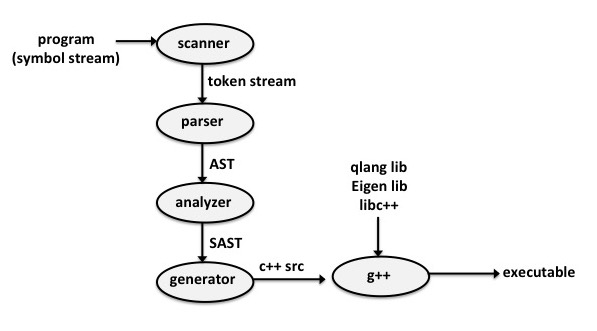
\includegraphics[scale=0.65]{architectural_diagram/architecture.jpg}
\end{center} 
\subsection{Components}
\begin{enumerate}
\item Scanner\\\\
The scanner was implemented using ocamellex - the associated file is scanner.mll. It was chiefly implemented by Christopher Campbell and Winnie Narang.\\\\
The scanner takes a program (symbol stream) as input and tokenizes it to produce a token stream. The tokenization process provides basic syntax checking, rejecting programs that contain illegal symbols and illegal combinations of symbols (e.g. the \$ symbol). Additionally, it discards information that is unnecessary for the remainder of the compilation process such as white space and comments.\\
\item Parser \& Abstract Syntax Tree\\\\
The parser was implemented using ocamlyacc - the associated files are ast.ml and parser.mly. It was chiefly implemented by Christopher Campbell and Sankalpa Khadka.\\\\
The parser takes the token stream produced by the scanner as input and parses it to produce an abstract syntax tree (AST), which describes the overall structure of the program. ast.ml provides parser.mly with the acceptable structure of the AST. The parsing process provides further syntax checking, rejecting programs that do not strictly meet the syntactic requirements of the AST (e.g. a malformed for statement).\\
\item Analyzer \& Semantically Analyzed Syntax Tree\\\\
The analzyer was implemented in OCaml - the associated files are analyzer.ml and sast.ml. Additionally, analyzer.ml utilizes ast.ml in order to be able to analyze its input. It was chiefly implemented by Christopher Campbell.\\\\
The analyzer takes the ast produced by the parser and analyzes it to produce a semantically analyzed abstract syntax tree (SAST). Like the AST, the SAST describes the overall structure of the program, but it also includes type information that was attached during the analysis process. sast.ml provides analyzer.ml with the acceptable structure of the SAST. The analysis process provides rigorous semantic checking, rejecting programs that violate type requirements (e.g. assigning a complex number to a variable declared as an integer), declaration requirements (e.g. using a variable that was not declared or attempting to declare a variable more than once), scope requirements (e.g. using a variable declared in another function), order requirements (e.g. calling a function before it is declared), and other language-specific requirements (e.g. not declaring a compute function). Additionally, the analyzer adds built-in information (i.e. built-in variables and functions) to the sast.\\
\item Generator\\\\
The generator was implemented in OCaml - the associated file is generator.ml. Additionally, generator.ml utilizes sast.ml in order to be able to process its input. It was chiefly implemented by Sankalpa Khadka, Jonathan Wong, and Winnie Narang.\\\\
The generator takes the sast produced by the analyzer and generates c++ code from it. Most of the code it generates is hard coded into generator.ml, but but it also draws on code from our standard library - qlanglib, libc++, and Eigen (a third-party library).\\
\item QLang Library\\\\
The QLang Library was implemented in c++ - the associated files are qlang.hpp and qlang.cpp. It was chiefly implemented by Jonathan Wong. The QLang library contains c++ code for carrying out some of the more complex conversions from qlang code to c++ code in the generator (e.g. generating qubits and carrying out the tensor product).
\end{enumerate}
\chapter{Test Plan}
  \section{Testing Phases}

\subsection{Unit Testing}
Unit testing was done at very frequent intervals, where each unit developed was tested rigorously using
multiple cases. The scanner,parse and the ast were tested in phase 1 and in the later phase the semantic
checker and the code generator were tested.


\subsection{Integration Testing}
In this phase,the various modules were put together and tested incrementally again. Initially the syntax of the
code was tested using multiple test cases and it was also ensured that only the correct syntax is
accepted by running multiple fail test cases. Later on, the semantic checker was integrated and the
semantics of the code were checked to be accurate without violating any of the rules of the language.
In the final phase the code generator was added to the system and was tested to generate the
corresponding C code. 

\subsection{System Testing}
System testing entailed end to end testing of our entire language framework. The input program written in QLang is fed to the compiler and it gives out the final output of the program, having passed through the parsing, scanning, compiling, code generation and execution phases. The final results were piped to an output file where we could see all the outputs.


\section{Automation and Implementation}
A shell script was written in order to automate the test cases at each level, syntax, semantic, code
generation and accurate execution. 
Our file is called runTests.sh, located in the 'test' folder. It takes a folder having QLang program files, and the operation to be done on them as arguments. The outputs of the respective operation can be seen in the corresponding output file. 


The operation options available are :

a : Parsing, scanning and AST generation.
s : SAST generation.
g : Code generation.
c : Generated code is compiled.
e : Generated executable is run, to generate the program's outputs. 

The operations mentioned above are each inclusive of the operations mentioned above them. That means, if you enter the 'g' option, runTests.sh will perform the tasks under 'a','s' and then the operations specific to 'g' as well.

The second argument is the folder that has the input program files. We have acronyms for two folder that are standard to our implementation, the SemanticSuccess and the SemanticFailures. So to run the sast generation on the files in SemanticSuccess folder, we would write :

sh runTests.sh s ss.

The entire code of this script can be seen in the appendix.


\section{Sample test programs}

The effort has been to exhaustively test every kind of execution scenario, in what can be a typical user program. We have created many test files to showcase varied kinds of programs that can be written in QLang, as can be seen in the contents of the SemanticSuccess and SemanticFailures folders.

The rationale is to make sure that syntactically or semantically incorrect programs are not compiled and echo corresponding meaningful error messages to the user, and that correct programs are accepted and executed correctly.

Hence, we have separate test programs to test all kinds of unary and binary operations on all datatypes that our language supports, and also for all kinds of statements and possible combinations of expressions. 
Though the test suite is too large to be included in this section, here are a few sample success and failure cases that showcase different applications of our language :


For instance, break_continue.ql is a QLang program as follows :

\begin{verbatim}

def func_test(int a) : int ret_name { 
        
        int i;

        for(i from 0 to 2 by 1)
        a=a+5;

        for(i from 2 to 0 by -1)
        {
            a=a*10;
            print(a);
            break;
        }

        for(i from 1 to 5)
        {
            print(a);
            continue;
            a=a*10;

        }

    ret_name = a;
}

def compute(): int trial {

   trial = func_test(20);
} 
\end{verbatim}

It generates break_continue.cpp as below upon passing it through the code generation code
\begin{verbatim}

#include <iostream>
#include <complex>
#include <cmath>
#include <Eigen/Dense>
#include <qlang>
using namespace Eigen;
using namespace std;
        
int func_test (int a )
{
	int i;
	int ret_name;
 

    for (int i = 0; i < 2; i = i + 1){
        	a = a + 5;

        }
    for (int i = 2; i < 0; i = i +   -1){
        
	{
	a = a * 10;

	cout << a << endl;

break;
	}

        }
    for (int i = 1; i < 5; i = i + 1){
        
	{
	cout << a << endl;

continue;
	a = a * 10;

	}

        }	ret_name = a;

	return ret_name;
}
int main ()
{
	int trial;
 
	trial = func_test(20);

	std::cout << trial << endl;

	return 0;
}
\end{verbatim}


and the generated output of this is :

\begin{verbatim} 
30
30
30
30
30
\end{verbatim}


Another example we consider is  mat\_qubit.ql


\begin{verbatim}
def func_test(mat a, mat b) : mat ret_name { 
        
        ret_name = a*b;

}


def compute(int a):mat trial {
	
	 mat zero;
	 mat one;

	 zero = |0>;
	 one  = |1>;

     trial = func_test(H,zero);
     printq(trial);

     trial = func_test(H,one);
     printq(trial);

}
\end{verbatim}

It generates mat\_qubit.cpp as below :


\begin{verbatim}
#include <iostream>
#include <complex>
#include <cmath>
#include <Eigen/Dense>
#include <qlang>
using namespace Eigen;
using namespace std;
        
MatrixXcf func_test (MatrixXcf a,MatrixXcf b )
{
	MatrixXcf ret_name;
 
	ret_name = a * b;

	return ret_name;
}
int main ()
{
	MatrixXcf zero;
	MatrixXcf one;
	MatrixXcf trial;
 
	zero = genQubit("0",0);
	one = genQubit("1",0);
	trial = func_test(H,zero);
	cout << vectorToBraket(trial) << endl;
	trial = func_test(H,one);
	cout << vectorToBraket(trial) << endl;

	std::cout << trial << endl;

	return 0;
}
\end{verbatim}

and it generates the qubits in the output as well, like :

\begin{verbatim}
(0.707107)|0> + (0.707107)|1>
(0.707107)|0> + (-0.707107)|1>
(0.707107,0)
(-0.707107,0)
\end{verbatim}

One more program we can show here is a demonstration of the capacity of the semantic analyzer to catch incorrect programs. For instance,

The program:

\begin{verbatim}
def func_test1(int z) : int ret_name { 
        int a;
        int b;
        int d;
        a = z;
        ret_name = z;

}
def func_test1(int z) : int ret_name2 { 

        ret_name2 = z;

}
def compute( int a):int trial {
      
      trial = func_test1(4);
}

\end{verbatim}


gives the error :
\begin{verbatim}
Fatal error: exception Analyzer.Except("Invalid function declaration: func_test1 was already declared")
\end{verbatim}


whereas the sample program

\begin{verbatim}
def func_test(float z) : float ret_name { 
        
        float a; 
        a = 5.8;
       
        ret_name = z;  
}
\end{verbatim}


would give the error :
\begin{verbatim}
Fatal error: exception Analyzer.Except("Missing 'compute' function")
\end{verbatim}

More such pass and fail test cases can be found in the appendix and in our project folder.






\chapter{Lesson Learned}
  \section{Sankalpa Khadka}
I realized that one of the important aspects of doing a big project is to make incremental progress, however small, over time. In the beginning, it is not always possible to have a global view of how each component of project fits in together. This can be discouraging factor at times, however this should not deter anyone from building the components of the project. Teamwork is very crucial to the success of the project. From the very beginning of the project, it is important to delegate responsibilities and making sure that each member of team is contributing to the project. Any disruption to this can affect the work balance.

Finally, it is a very fulfilling experience to design a programming language from CS perspective. This experience draws from both theory and application aspect of CS. Everyone doing similar projects in future should try to participate, contribute and enjoy the process.

\chapter{Appendix}
\appendix
\chapter{More on Quantum Computing}\label{app:quantum:more}
  \section {Common quantum gates}

\subsubsection*{Pauli Operators}
	The \emph{Pauli operators} are the special single qubit gates which are represented by the Pauli matrices $\{I, X, Y, Z\}$ as follows
	\[
I =
\begin{bmatrix}
 1 & 0  \\
 0 & 1  
\end{bmatrix}
\qquad
X =
\begin{bmatrix}
 0 & 1  \\
 1 & 0  
\end{bmatrix}
\qquad
Z =
\begin{bmatrix}
 1 & 0  \\
 0 & -1  
\end{bmatrix}
\qquad
Y =
\begin{bmatrix}
 0 & -i  \\
 i & 0  
\end{bmatrix}.
\]
For example, the application of $X$ causes bit-flip in following ways:
\[
X\ket{0}=\begin{bmatrix}
 0 & 1  \\
 1 & 0  
\end{bmatrix}
\begin{bmatrix}
 1   \\
 0   
\end{bmatrix}=\begin{bmatrix}
 0   \\
 1   
\end{bmatrix}= \ket{1}
\]
\[
X\ket{1}=\begin{bmatrix}
 0 & 1  \\
 1 & 0  
\end{bmatrix}
\begin{bmatrix}
 0   \\
 1   
\end{bmatrix}=\begin{bmatrix}
 1   \\
 0   
\end{bmatrix}= \ket{0}.
\]
\subsubsection*{Hadamard Gate}
The \emph{Hadamard gate} is defined by the matrix:
\[
H= \frac{1}{\sqrt{2}}\begin{bmatrix}
 1 & 1  \\
 1 & -1
\end{bmatrix}.
\]
The Hadamard gate maps the computational basis states into superposition of states. The Hadamard gate is significant since it produces maximally entangled states from basis states in the following ways:
\[
H\ket{0}=\frac{1}{\sqrt{2}}(\ket{0}+\ket{1})
\qquad
H\ket{1}=\frac{1}{\sqrt{2}}(\ket{0}-\ket{1}).
\]

\subsubsection*{Controlled-U Gates}
	A \emph{controlled-U gate} is the quantum gate in which the $U$ operator acts on the \new{$n$\textsuperscript{th} $n$-qubit} only if the value of the preceeding qubit is $1$.\\ For example: In a Controlled-\textsf{NOT} gate, the \textsf{NOT} operator flips the second qubit if the first qubit is $1$.
	\[
	\textsf{CNOT} = \begin{bmatrix}
 1&0&0&0\\
0&1&0&0\\
0&0&0&1 \\
0&0&1&0\end{bmatrix}
	\]
	
	\[
	\textsf{CNOT}\ket{00}=\ket{00}
	\]
	\[
	\textsf{CNOT}\ket{01}=\ket{01}
	\]
	\[
	\textsf{CNOT}\ket{10}=\ket{11}
	\]
	\[
	\textsf{CNOT}\ket{11}=\ket{10}.
	\]
	
	
\section {Tensor product and its properties}

Let $A=(a_{i,j})$ be a matrix with respect to the ordered basis $\mathcal{A}=(u_1,\dots,u_n)$ and $B=(b_{i,j})$ be a matrix with respect to the ordered basis $\mathcal{B}=(v_1,\dots,v_m)$. Consider the ordered basis $\mathcal{C}=(u_i \otimes v_j)$ ordered by lexicographic order, that is $u_i \otimes v_j \leq u_l \otimes v_k$ if if $i<l$ or $i=l$ and $j<k$. The matrix of $A \otimes B$ with respect to $\mathcal{C}$ is : 
\[
	A \otimes B= 
	\begin{bmatrix}
 	a_{1,1}B & a_{1,2}B & \dots & a_{1,n}B\\
	a_{2,1}B & a_{2,2}B & \dots & a_{2,n}B\\
	\vdots & \vdots & \ddots & \vdots \\
	a_{n,1}B & a_{n,2}B & \dots & a_{n,n}B
	\end{bmatrix} 
\]
		This matrix is called the tensor product of the matrix $A$ with the matrix $B$.
\begin{itemize}
\item $A \otimes B \otimes C =  (A \otimes B ) \otimes C = A \otimes (B \otimes C)$
\item $ a ( \ket{x} \otimes \ket{y}) = a \ket{x} \otimes \ket{y} = \ket{x} \otimes a\ket{y}$
\item $ ( A \otimes B) \cdot (\ket{y}\ket{z}) = A\ket{y} \otimes B\ket{z}$
\item $ ( A \otimes B) \cdot ( C \otimes D) = AC \otimes BD$
\item $ (A \otimes B) ^{H} = A^{H} \otimes B^{H}$
\item If $ A$ and $B$ unitary, $A \otimes B$ is unitary.
\item If $\ket{x}=\ket{x_1} \ket{x_2}$ and $\ket{y}=\ket{y_1}\ket{y_2}$ then $\dotproduct[x,y]=\dotproduct[x_1,y_1] \dotproduct[x_2, y_2]$ 
\end{itemize}

\chapter{Source Code}

\end{document}
